\begin{figure}[H]
  \centering
  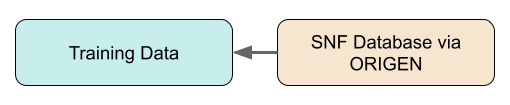
\includegraphics[width=0.7\linewidth]{./chapters/exp1/methodology1_1.png}
  \caption[First portion of the flowchart from Figure \ref{fig:method1}]
          {First portion of the flowchart from Figure \ref{fig:method1} being 
           described in this section.}
\end{figure}

Of interest to an entity trying to create a weapon is partially irradiated fuel
if they have plutonium separations capabilities or any radioactive substance in
the case of a dirty bomb. Thus, this work focuses on \gls{SNF} from commercial
power reactors. Ideally, a large enough database of \gls{SNF} nuclide assays
would be able to be used for this work. Since that does not exist, the 
database will be simulated via \gls{ORIGEN} \cite{origen, origenarp}.  

\subsection{Simulation Fidelity}
\label{sec:fidelity}

Nuclear fuel cycle studies involve tracking the material flow of nuclear fuel.
This can be anywhere from mining to waste management, or focus on a process
step in between. Fuel cycle studies are not necessarily nuclear-specific. For
example, they can be used to evaluate economic predictions, environmental
impact, transportation planning, etc.  In order to draw conclusions from these
studies, it is common to use a nuclear fuel cycle simulator that tracks the
quantities of interest. These allow the comparison of different fuel types,
reactor technologies, material processing steps, etc. 

There are simplifications researchers need to make in order to experiment in a
controlled way. Fuel cycle simulators, built for a specific needs, must remove
complicating factors that are less relevant to the study.  For example, one
tool might be suited well to large-scale systems analysis with little nuclear
physics included in the models, and another might focus on detailed isotopics
within a system to track plutonium.

Because a large portion of a nuclear forensics investigation relies on
measuring isotopics, this work used \gls{ORIGEN} \cite{origen}, which is a part
of the \gls{SCALE} 6.2 modeling and simulation suite of computational tools
developed for nuclear design and safety \cite{scale}. \gls{ORIGEN} was chosen
for its physically detailed models of activation, depletion, and decay.
Specifically, the ARP module of the code was used: \gls{ORIGEN-ARP}
\cite{origenarp}.

\gls{ORIGEN} calculates time-dependent nuclide concentrations (or quantities
derived from these) that result from activation and depletion calculations. The
physics (i.e., neutron transport and decay) calculations are carried out in
other \gls{SCALE} modules that solve the depletion equations.  This generates
libraries for \gls{ORIGEN} that include the probabilities of reaction (i.e.,
cross sections) for the system.

To obtain an \gls{SNF} recipe from a reactor simulation, \gls{ORIGEN} uses the
desired input power generation with the cross section library to calculate a
flux, the resulting depletion, and the end composition (i.e., isotopic recipes
or nuclide vectors).  Another output is decay; the composition is computed
using decay equations with nuclear data \cite{endf}. These compositions provide
source terms for other calculations, such as decay emission spectra from
neutrons, alpha particles, beta particles, and gamma rays. Other derived
quantities like activity, decay heat, or radiological hazard factors are also
an option.

\begin{table}[!htbp]
  \centering
  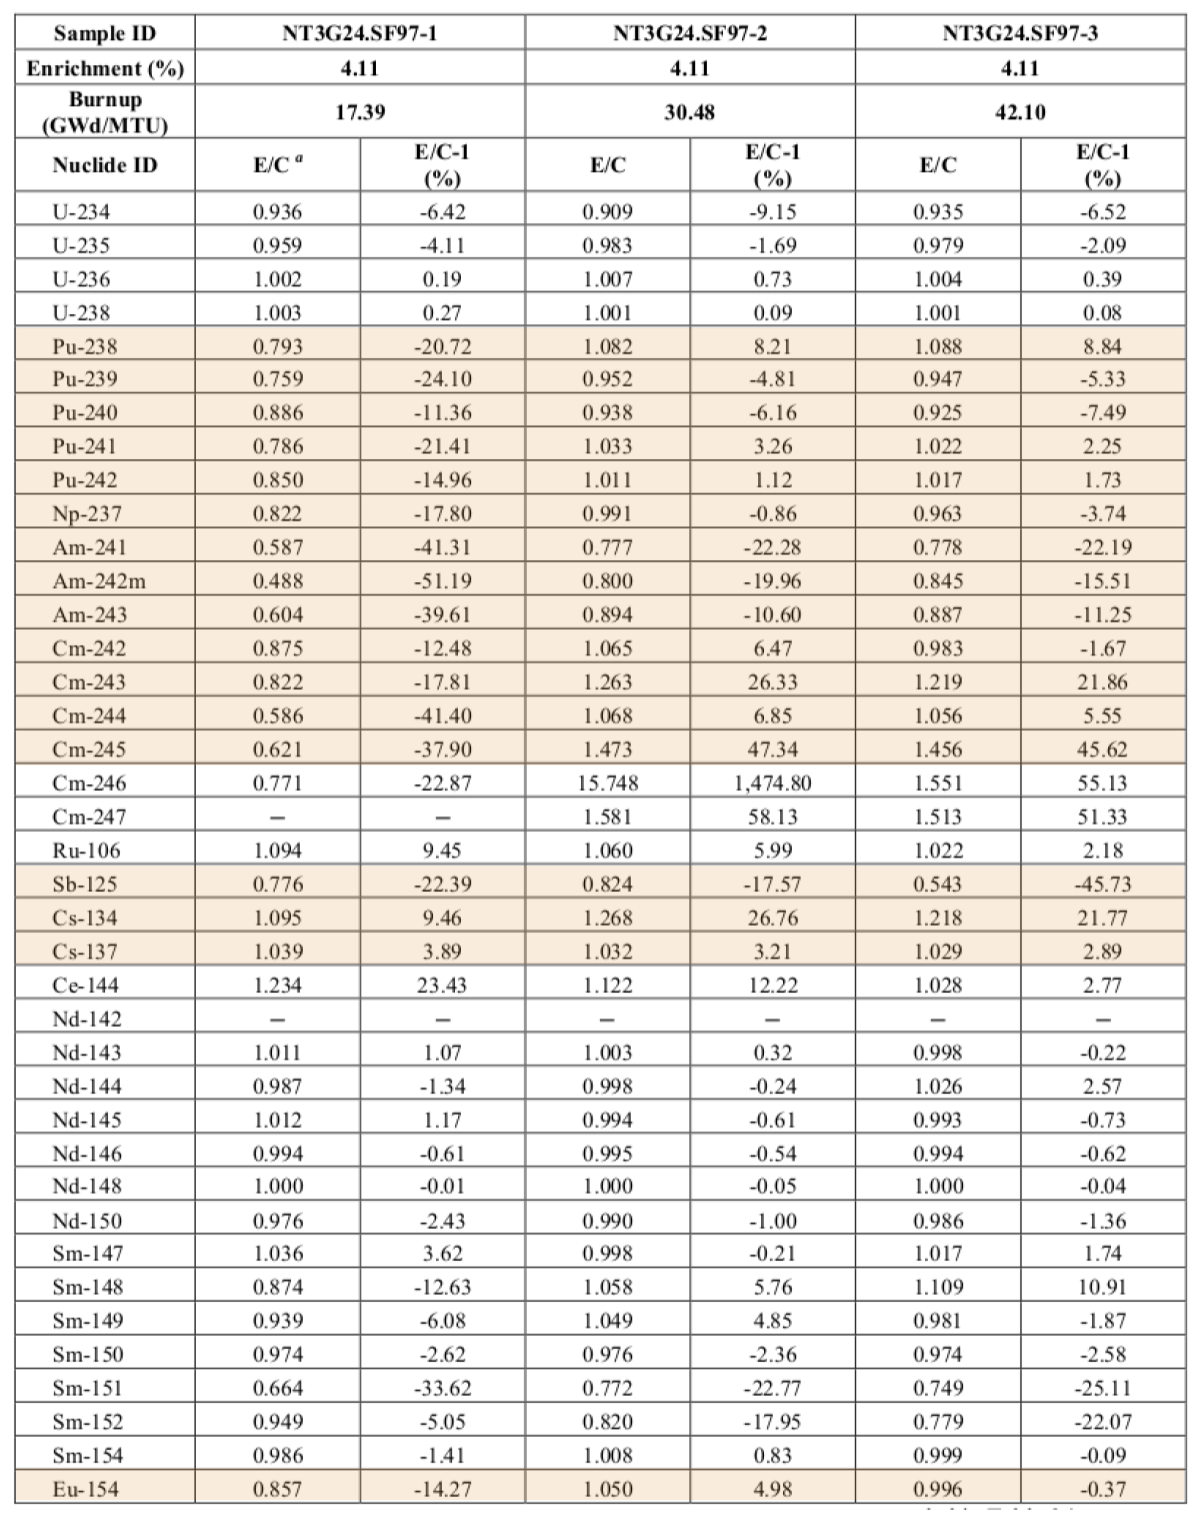
\includegraphics[width=\linewidth]{./chapters/exp1/pwr_benchmark.png}
  \caption[Example of \acrshort{SCALE} simulation benchmarking results]
          {Example set of results from work that uses \acrshort{SFCOMPO} test 
           cases for \acrshort{PWR} simulation benchmarking of \acrshort{SCALE} 
           in Reference \cite{pwr_benchmark_2010}.}
  \label{tbl:pwr_bench}
\end{table}

\gls{ORIGEN-ARP} allows users to access a wider range of simulations by
interpolating between the pre-calculated libraries instead of creating new
libraries.  The libraries contained in \gls{ORIGEN-ARP} for various reactor
technologies and fuel assemblies are optimized to sets of \gls{U235}
enrichments for the relevant coolant and moderator densities.  They also
contain optimized burnup steps, which informed the burnup steps used in this
work \cite{origenarp}.  The \gls{SNF} simulated in this work comes from a
homogenized reactor core, and so does not take axial variations of burnup into
account.  Through \gls{ORIGEN}, given an initial material composition, some
reactor operation parameters, and a reactor type, one can quickly perform many
different nuclear reactor simulations and obtain \gls{SNF} recipes. Since there
are nearly 500k simulations being used in this work, \gls{ORIGEN-ARP} is able
to provide these simulations with relative computational ease. 

Of course, there may be some losses in simulation fidelity by taking this
route.  \gls{ORIGEN-ARP} is well-validated for \gls{LWR} \gls{SNF}
\cite{lwr_valid}.  Additionally, recycled \gls{SNF} in the form of mixed oxide
fuel has been benchmarked for the relevant reactors \cite{mox_valid}.  Still,
there are some nuclides for which simulations are not well-matched to the
experimental measurements. The systematic overprediction of Eu154 is documented
in Reference \cite{skutnik_eu154}.  Some details of computed versus
experimental nuclide compositions for \gls{PHWR}s are covered in Reference
\cite{skutnik_2021}. Table \ref{tbl:pwr_bench} shows a small slice of the
results in Reference \cite{pwr_benchmark_2010}.  This work uses several
\gls{SCALE} modules to simulate nuclide measurements, and using a former
release of \gls{SFCOMPO} \cite{sfcompo, valid_sfco}, compares these to the
experimental measurements.  Although \gls{ORIGEN-ARP} was not used, some
reactor core simplifications were made, where the target fuel rod had
individual mixtures specified and the remainder of the core was homogenized.
The $\frac{E}{C}$ in the table refers to the experimental to calculated ratio
of each measurement, for which there are three sets of comparisons (labeled at
the top by "Sample ID").  The highlighting is for nuclides that are in one or
both of the experiments in this work, and tend to have larger errors.  The
first sample is a lower burnup and has the largest errors.

In summary, it is important to note that that the simulated training set as
ground truth is not perfect truth, for some nuclides more than others.  The
prediction performance will be impacted by the poorly simulated nuclides, but a
detailed study on  which nuclide measurements to exclude is outside of the
scope of this work.

\subsection{Training Set Labels}
\label{sec:snflbls}

The design of the training set is dependent on a number of factors.  First, it
must have a sufficient number of burnup sets and time since irradiation steps
to provide robust prediction. This is chosen by maximizing the steps for both
parameters, while balancing the computational limitations of a large training
set. Through previous experience, an approximate limit would be around $10^6$
database entries for the specific calculations in this work and employing
reasonable computational limitations.

\begin{table}[!htb]
  \centering
  \begin{subtable}{\linewidth}
    \centering
    \begin{tabular}{@{}lll@{}}
    \toprule
      \textbf{PWR} & \textbf{BWR}  & \textbf{PHWR} \\ \toprule
      CE14x14      & GE7x7-0       & CANDU19       \\
      W17x17       & Abb8x8-1      & CANDU28       \\
      S18x18       & Atrium10x10-9 & CANDU37       \\
      BW15x15      & SVEA64-1      &               \\
      VVER440      &               &               \\ \bottomrule
    \end{tabular}
    \caption{\acrshort{ORIGEN} designations for reactor technologies and fuel assembly design.}
    \label{tbl:rxtrtype}
    \vspace*{5mm}
  \end{subtable}
  \begin{subtable}{\linewidth}
    \centering
    \begin{tabular}{@{}llll@{}}
      \toprule
                                & \textbf{PWR}              & \textbf{BWR}              & \textbf{PHWR} \\ \toprule
      Power Density [MW/MTU]    & 25, 35, 41                & 10, 22                    & 2.2, 18, 22   \\
      Burnup [GWd/MTU]          & 2--68                     & 1--68                     & 0.45--12.6    \\
      Moderator Density [g/cc]  & 0.71                      & \{0.1, 0.3, 0.5, 0.7\}    & 0.84          \\
      Enrichment [\% \gls{U235}]& \{0.5, 1.5, 2, 3, 4, 5\}  & \{0.5, 1.5, 2, 3, 4, 5\}  & 0.711         \\
      Cooling Time [days]       & \multicolumn{3}{c}{\{0--6000\} in 100-day steps}                      \\ \bottomrule
    \end{tabular}
    \caption{Simulation parameters for \acrshort{ORIGEN} input files.}
    \label{tbl:rxtrparam}
  \end{subtable}%
  \caption[Training set database design for \acrshort{ORIGEN} input files.]
          {Training set database design and parameters for \acrshort{ORIGEN} 
           input files.}
  \label{tbl:train}
\end{table}

Secondly, the training set must represent what exists in the real world. This
was accomplished by studying the spread of parameters in the \gls{SFCOMPO}
database \cite{sfcompo, valid_sfco}.  To ensure this, a variety of reactor
types and assembly designs were included, listed in Table \ref{tbl:rxtrtype}.
Table \ref{tbl:rxtrparam} lists the rest of the simulation inputs. These
include not only the labels of prediction interest, \gls{U235} enrichment,
burnup, and time since irradiation, but also other important simulation input
parameters such as the reactor power density and the moderator density.  (Water
is both the moderator and coolant in all simulated reactor types.)

\begin{figure}[!hbt]
  \makebox[\textwidth][c]{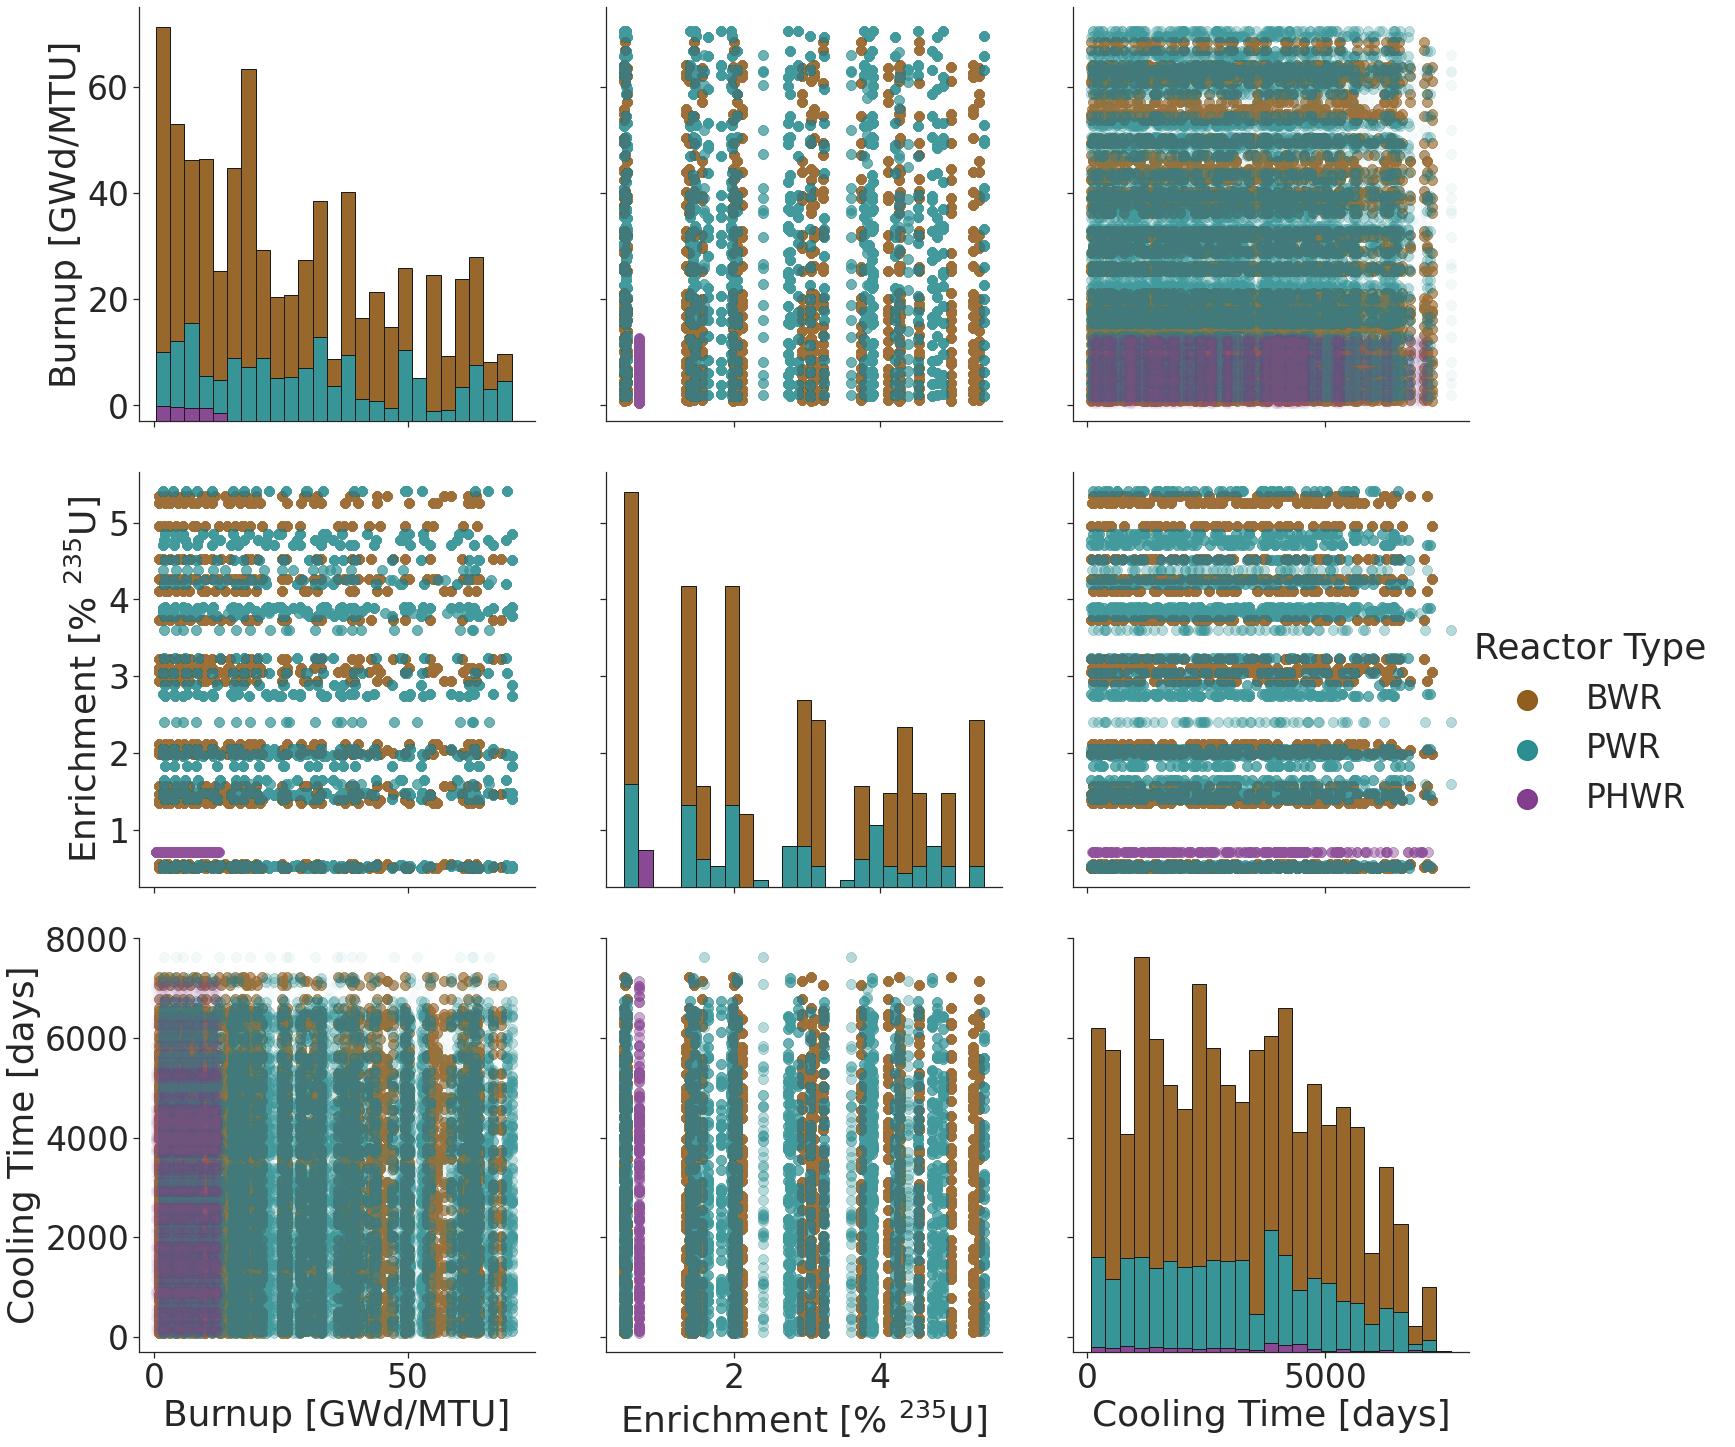
\includegraphics[width=\linewidth]{./chapters/exp1/histogram_scatter_trainset_viz.png}}
  \caption[Visualization of training set labels distributions]
          {A combination of histograms and scatter plots to visualize the 
           distribution of prediction labels in the training set.}
  \label{fig:trainhist}
\end{figure}

The third factor influencing database design is \gls{ML} algorithm performance.
As mentioned in Section \ref{sec:errs}, many algorithms are developed with the
assumption that the training set will be \acrfull{i.i.d.}.  This is important
so that the model does not overvalue or overfit a certain area in the training
space. With the training set design, there are predetermined values for
enrichment, burnup, and time since irradiation.  While there are $21-28$ burnup
steps \todo{add full lists?} (depending on the reactor type) and 61 cooling
time steps, there are only 6 values for enrichment. This creates the risk that
the algorithm will end up being unable to generalize outside of those discrete
values. Therefore, the burnup steps and time steps are perturbed randomly in a
range that is $\pm10\%$ and $\pm30\%$ from the originally defined values,
respectively.  The enrichment also gets perturbed by $\pm10\%$, and not more
because the cross-section libraries in \gls{ORIGEN-ARP} are pre-calculated for
those enrichment values, so deviating too far from them would result in
inaccurate \gls{SNF} simulations. The power densities and moderator densities
were kept at the values defined in Table \ref{tbl:rxtrparam}.  Additionally,
natural variations in ${}^{234}\text{U}$ and ${}^{236}\text{U}$ were not
considered.  The percentage of the two uranium isotoped in fresh fuel were kept
the same for all \gls{SNF} simulations: 0.0356\% for ${}^{234}\text{U}$ and
0.0184\% for ${}^{236}\text{U}$.  The 0-valued burnup and cooling time entries
were then filtered out so that the future calculations of relative error would
be possible for all predictions.  

The resulting training set is $450240$ (or $4.5 \times 10^5$) entries.  Figure
\ref{fig:trainhist} visualizes the somewhat even distribution of the burnup and
cooling time parameters, and shows the lack of even distribution of the
enrichment parameter through a combination of scatter plots and histograms.
Note that there are many more \gls{BWR}s present in the histograms because of
the multiple moderator densities simulated (see Table \ref{tbl:rxtrparam}). The
number of \gls{PWR}, \gls{BWR}, and \gls{PHWR} entries in the training set is
120960 (26.8\%), 322560 (71.6\%), and 6720 (1.5\%), respectively.

\subsection{Training Set Features}
\label{sec:snffeats}

The other design decision regarding the training set is related to
which nuclides to track, i.e., the features.  For this experiment, nuclide
masses are necessary, and the most common measurements in \gls{SFCOMPO} guide
the list of nuclides tracked.  

The set of training features of 29 nuclide masses listed in Table
\ref{tbl:nucmass} was designed with the following reasons in mind.  First, the
training set feature measurement units are chosen to be convertable to those
present in the external, real-world test set: the \gls{SFCOMPO} database.  The
\gls{ORIGEN} simulations output the nuclide masses in grams, $g$, and they are
converted to the units of milligrams per gram of initial uranium, $mg/gU_i$,
when the models are externally tested against \gls{SFCOMPO}.  Second, the 29
nuclides chosen were based on the presence of measurements in \gls{SFCOMPO},
where these were present in at least 100 of the samples in the database.  The
external test set is described in more detail in Section \ref{sec:sfcompo}.
These choices are made so that the training set entries mimic a full assay
being done via mass spectrometry techniques, and thus represents what this work
refers to as "perfect knowledge" scenario.  

\begin{table}[!htb]
  \centering
  \begin{tabular}{@{}|l|l|l|l|l|l|l|l|@{}}
    \hline
    \allbold{${}^{241}\text{Am}$} & ${}^{242m}\text{Am}$ &
    \allbold{${}^{243}\text{Am}$} & ${}^{242}\text{Cm}$ &
    \allbold{${}^{244}\text{Cm}$} & \allbold{${}^{134}\text{Cs}$} &
    \allbold{${}^{137}\text{Cs}$} & \allbold{${}^{154}\text{Eu}$} \\  
    \hline
    ${}^{143}\text{Nd}$ & ${}^{144}\text{Nd}$ & ${}^{145}\text{Nd}$ &
    ${}^{146}\text{Nd}$ & ${}^{148}\text{Nd}$ & ${}^{150}\text{Nd}$ &
    \allbold{${}^{237}\text{Np}$} & \allbold{${}^{238}\text{Pu}$} \\ 
    \hline
    \allbold{${}^{239}\text{Pu}$} & \allbold{${}^{240}\text{Pu}$} &
    ${}^{241}\text{Pu}$ & ${}^{242}\text{Pu}$ & ${}^{147}\text{Sm}$ &
    ${}^{149}\text{Sm}$ & ${}^{150}\text{Sm}$ & ${}^{151}\text{Sm}$ \\ 
    \hline
    ${}^{152}\text{Sm}$ & \allbold{${}^{234}\text{U}$} &
    \allbold{${}^{235}\text{U}$} & ${}^{236}\text{U}$ & ${}^{238}\text{U}$ &  &
    & \\  
    \hline
  \end{tabular}
  \caption[Set of nuclide features for first experiment]
          {Set of features saved for the first experiment, nuclide masses 
           measured in $grams$. The bold nuclide masses overlap with the 
           nuclides in Table \ref{tbl:nucacts}.}
  \label{tbl:nucmass}
\end{table}

% Edit: None of the algs are dependent on feature distributions, so leaving out

%Many \gls{ML} algorithms are dependent on a presumed feature distribution.
%Figure \ref{fig:nucshist} is a set of histograms for each feature, showing the
%spread of each nuclide mass measurement across the entire training set.  While
%a few nuclides have a normal distribution (the most common presumption), many
%do not. Fortunately, both \textit{k}-nearest neighbors and decision trees are
%non-parametric methods that do not make any underlying assumptions about
%feature probability distributions. The \gls{MLL} method, however, does make the
%assumption of a normal distribution. Any poor performance could therefore be
%explained by this underlying assumption being an inaccurate representation of
%the features in the training set.
%
%\begin{figure}[!htb]
%  \makebox[\textwidth][c]{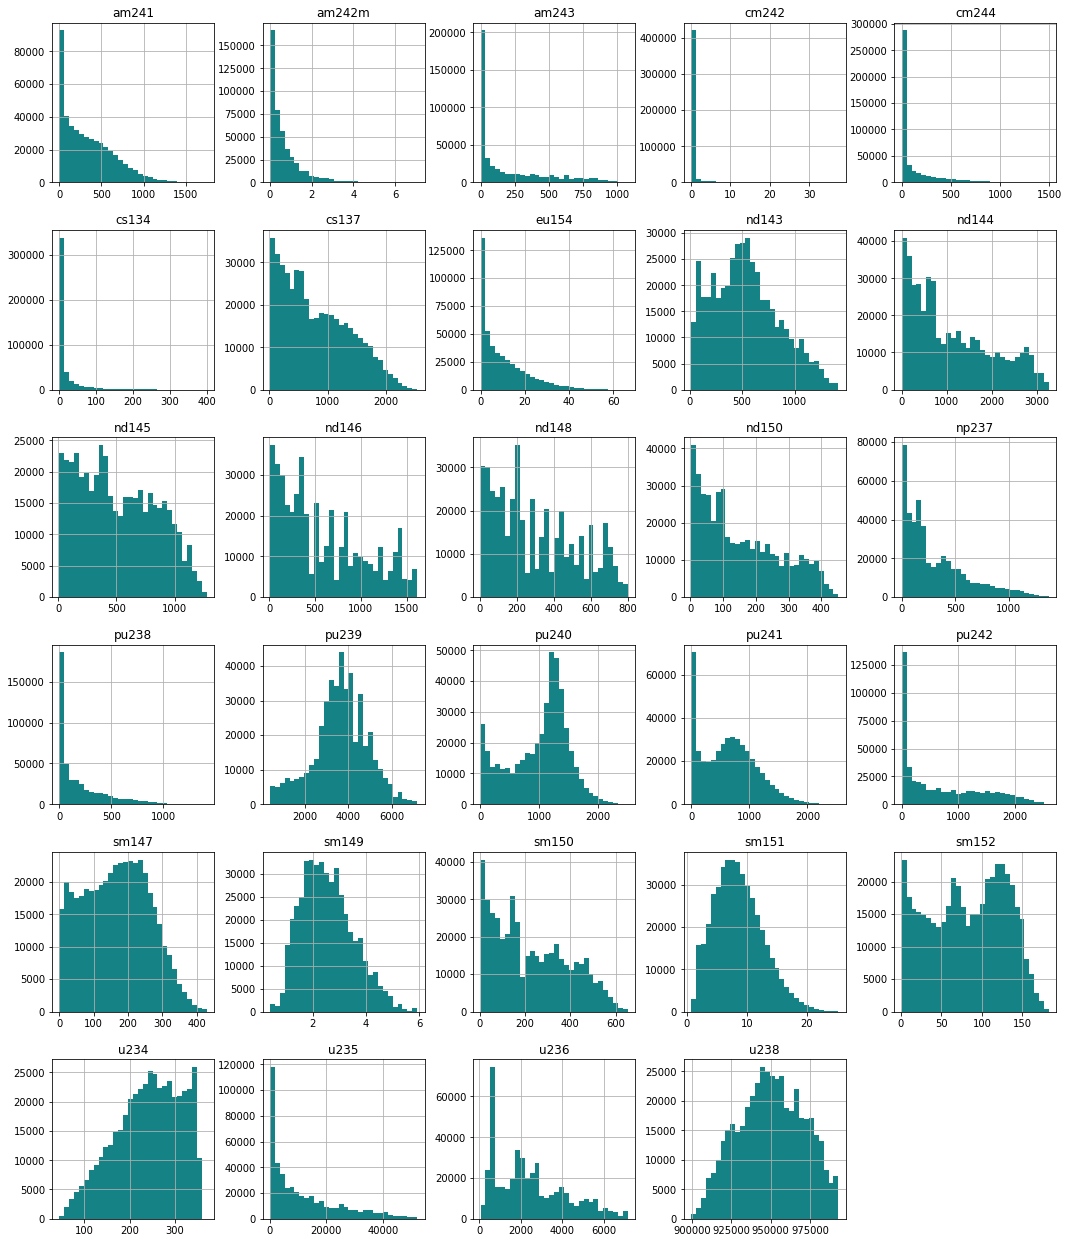
\includegraphics[width=\linewidth]{./chapters/exp1/histograms_trainset_features_nucs.png}}
%  \caption{Histograms of each of the 29 nuclide masses.}
%  \label{fig:nucshist}
%\end{figure}

